% Created 2021-01-24 Sun 22:49
% Intended LaTeX compiler: pdflatex
\documentclass[11pt]{article}
\usepackage[utf8]{inputenc}
\usepackage[T1]{fontenc}
\usepackage{graphicx}
\usepackage{grffile}
\usepackage{longtable}
\usepackage{wrapfig}
\usepackage{rotating}
\usepackage[normalem]{ulem}
\usepackage{amsmath}
\usepackage{textcomp}
\usepackage{amssymb}
\usepackage{capt-of}
\usepackage{hyperref}
\usepackage{minted}
\hypersetup{colorlinks=true, linkcolor=black, filecolor=red, urlcolor=blue}
\usepackage[turkish]{babel}
\author{Eren Hatırnaz}
\date{25 Mayıs 2020}
\title{Yazılım Gündemi - 2020/20\\\medskip
\large 18-24 Mayıs 2020}
\hypersetup{
 pdfauthor={Eren Hatırnaz},
 pdftitle={Yazılım Gündemi - 2020/20},
 pdfkeywords={},
 pdfsubject={},
 pdfcreator={Emacs 27.1 (Org mode 9.3)},
 pdflang={Turkish}}
\begin{document}

\maketitle
\tableofcontents \clearpage\shorthandoff{=}

\begin{center}
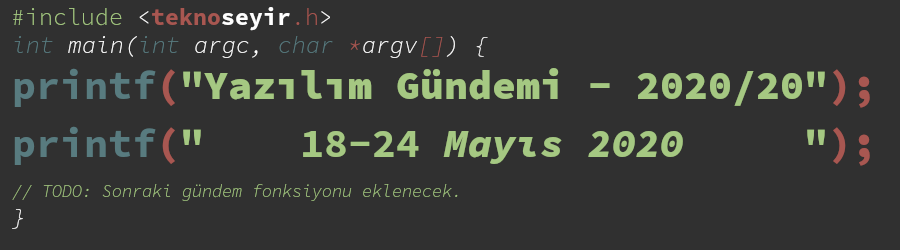
\includegraphics[width=.9\linewidth]{gorseller/yazilim-gundemi-banner.png}
\end{center}

\begin{center}
\href{../19/yazilim-gundemi-2020-19.pdf}{< Önceki Gündem} | \textbf{18-24 Mayıs 2020} | \href{../21/yazilim-gundemi-2020-21.pdf}{Sonraki Gündem >}

\href{https://teknoseyir.com/blog/yazilim-gundemi-2020-20}{TeknoSeyir'de Oku}
\end{center}

\section{C\# \href{https://devblogs.microsoft.com/dotnet/welcome-to-c-9-0/}{9.0 sürümü yayınlandı}}
\label{sec:org45ab6aa}
Microsoft'un geliştiriciler için özel olarak düzenlediği etkinliği olan BUILD
bu yıl koronavirüs nedeniyle sanal olarak düzenlendi. Geçtiğimiz hafta
düzenlenen BUILD 2020 etkinliğinde .NET ekosistemi altında geliştirilen
programlama dili C\#'ın da 9.0 numaralı sürümü yayınlandı. Her ne kadar uzun
bir süredir .NET ekosisteminden uzak kalmış olsam da C\# ilk göz ağrılarımdan
biridir. Programlama başlarken kullandığım dillerden biri olması dolayısıyla
yapısı hakkında bilgim var. Bu sürümle birlikte gelen birkaç özelliği birlikte
inceleyelim:

\subsection{Init-only properties}
\label{sec:org2911119}
Nesne yönelimli programlama dili olmasından dolayı verileri nesne olarak
temsil etme özellikleri oldukça gelişmiş olan C\#'da halihazırda bu şekilde
basit bir sınıf oluşturup kullanabiliyorduk:

\begin{minted}[breaklines=true,breakanywhere=true,frame=lines, linenos, label=C\#]{csharp}
public class Kisi
{
    public string Ad { get; set; }
    public string Soyad { get; set; }
}

new Kisi
{
    Ad = "Eren",
    Soyad = "Hatırnaz"
}
\end{minted}

Fakat bazı durumlarda bazı property'lerin tanımlandıktan sonra
değiştirilememesini isteyebiliriz. İşte bu durumda imdadımıza init-only
propert'ler yetişiyor ve bu şekilde bir tanımlama ile isteğimizi
gerçekleştirebiliyoruz:
\begin{minted}[breaklines=true,breakanywhere=true,frame=lines, linenos, label=C\#]{csharp}
public class Kisi
{
    public string Ad { get; init; }
    public string Soyad { get; init; }
}
\end{minted}
\subsection{Records}
\label{sec:org77e4469}
Eğer yukarıdaki kullanımın askine birkaç property'yi değil tüm objeyi
immutable yapmak istiyorsanız o zaman da yardımımıza yeni Records özelliği
koşuyor:
\begin{minted}[breaklines=true,breakanywhere=true,frame=lines, linenos, label=C\#]{csharp}
public data class Kisi
{
    public string Ad { get; init; }
    public string Soyad { get; init; }
}
\end{minted}
Tanımladığınız sınıfı \texttt{public data class} olarak işaretlediğinizde o artık
bir Record haline gelmiş oluyor ve artık bir kere oluşturduğunuz bir record
objesini bir daha değiştiremiyorsunuz, onun yerine artık bu şekilde var olan
objenin özelliklerini değiştirip yeni objeler oluşturarak devam ediyorsunuz:
\begin{minted}[breaklines=true,breakanywhere=true,frame=lines, linenos, label=C\#]{csharp}
var digerKisi = person with { Ad = "Ahmet" }
\end{minted}
Daha önce "Ad=Eren, Soyad=Hatırnaz" olarak tanımladığımız objeyi kullanarak
"Ad=Ahmet, Soyad=Hatırnaz" şeklinde yeni bir obje oluşturmuş olduk.

Immutable konusu benim de zaman zaman kafamı karıştıran bir konu, dolayısıyla
bu tarz kullanımların tam olarak hangi sorun için bir çözüm olduğunu
bilemiyorum ama takip ettiğim kadarıyla topluluk bu özellikler için sevinmiş
durumda.
\subsection{Top-level programs}
\label{sec:org389c5e8}
Diğer birçok programlama dilinden de alışık olduğumuz üzere C\#'da basit bir
programın yapısı şöyle oluyor genelde:
\begin{minted}[breaklines=true,breakanywhere=true,frame=lines, linenos, label=C\#]{csharp}
using System;

class Program
{
    static void Main()
    {
        Console.WriteLine("Merhaba Dünya");
    }
}
\end{minted}
Fakat artık daha da basit şekilde, Python ve Ruby gibi dillerden aşılık
olduğumuz gibi bu şekilde de uygulamalar yazabileceğiz:
\begin{minted}[breaklines=true,breakanywhere=true,frame=lines, linenos, label=C\#]{csharp}
using System;

Console.WriteLine("Merhaba Dünya");
\end{minted}

C\# 9.0 ile birlikte gelen diğer özellikler ve detaylar için konu başlığına
eklediğim bağlantıya tıklayabilirsiniz. Ayrıca geçtiğimiz hafta içerisinde
\href{https://devblogs.microsoft.com/dotnet/announcing-net-5-preview-4-and-our-journey-to-one-net/}{.NET 5 Preview 4} sürümü de duyuruldu.
\section{Microsoft yeni platformlar arası uygulama geliştirme \href{https://devblogs.microsoft.com/dotnet/introducing-net-multi-platform-app-ui/}{çözümünü tanıttı}: \href{https://github.com/dotnet/maui}{.NET Multi-platform App UI}}
\label{sec:orga47134b}
Microsoft'un 2016 yılında .NET için açık kaynaklı teknolojiler üreten Xamarin
\href{https://blogs.microsoft.com/blog/2016/02/24/microsoft-to-acquire-xamarin-and-empower-more-developers-to-build-apps-on-any-device/}{firmasını satın almıştı}. Xamarin tarafından geliştirilen Xamarin.Forms'da
doğal olarak Microsoft'a geçmiş oldu. İşte bu satın almanın yeni meyvesi
olacak şey de bugün konuşacağımız .NET Multi-platform App UI oldu.

\begin{center}
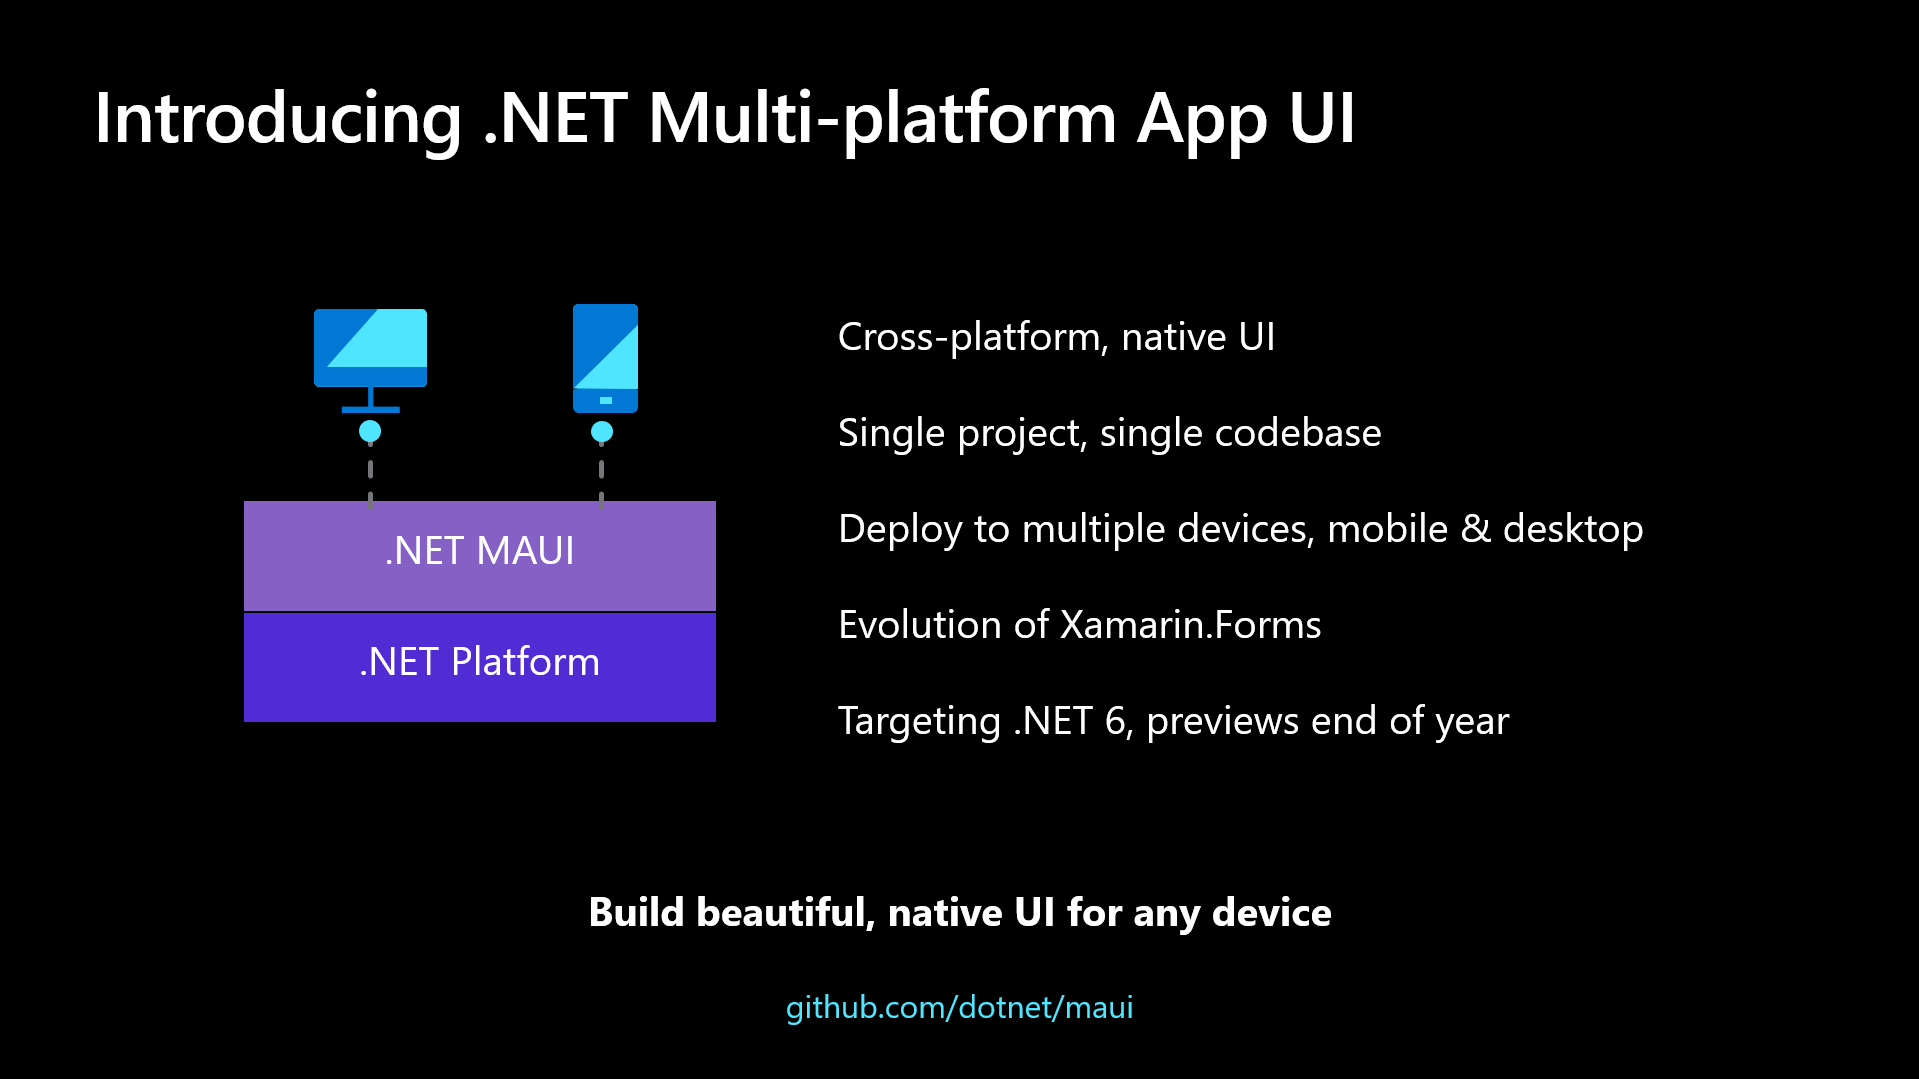
\includegraphics[width=.9\linewidth]{gorseller/dotnet-multiplatform-app-ui.png}
\end{center}

\href{https://github.com/xamarin/xamarin.forms}{Xamarin.Forms} hatırlamayan ya da bilmeyenler için .NET ekosistemi içerisinde
platformlar arası (cross-platform) uygulama geliştirmeye yarayan bir
teknoloji. Geçtiğimiz hafta içerisinde ise bu teknolojinin artık evrimleşip
başka bir teknolojiyle birleşme vaktinin geldiğini duyuruldu. .NET MAUI,
kısaca Xamarin.Forms'un evrimleşmiş ve gelişmiş halidir diyebiliriz.
Microsoft, henüz erken geliştirilme aşamasında olan bu teknolojisi ile biz
geliştiricilere tek bir projeden hem Windows hem macOS hem de iOS ve Android
uygulaması çıkarmayı vaat ediyor.

\begin{figure}[htbp]
\centering
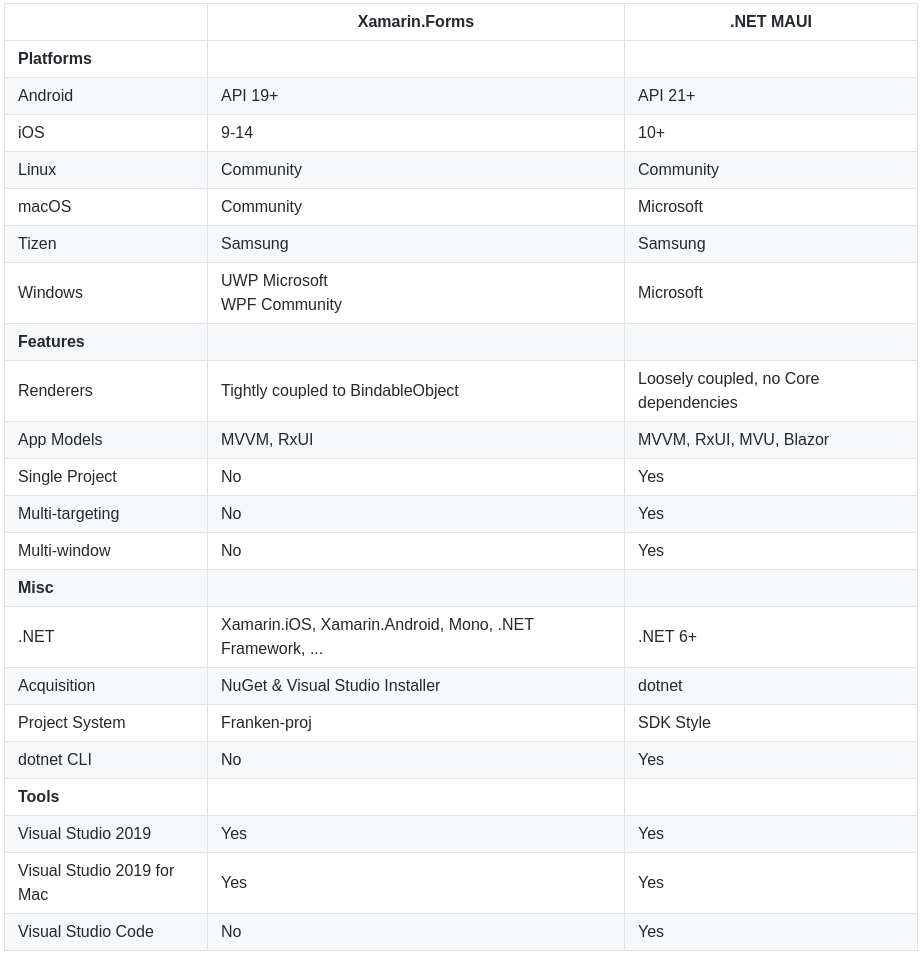
\includegraphics[width=.9\linewidth]{gorseller/dotnet-maui-vs-xamarin-forms.png}
\caption{Xamarin.Forms ve .NET MAUI arasındaki farklar tablosu}
\end{figure}

.NET 6 sürümüyle birlikte hayatımıza girmesi planlanan bu teknolojiyle
birlikte MVVM (Model-View-ViewModel) ve RxUI gibi Design Pattern ve uygulama
modellerinin yanı sıra .NET MAUI, MVU(Model-View-Update) ve Blazor gibi
yapıları da destekleyecek.

Peki bu gelişmeler Xamarin ve Xamarin.Forms için ne anlama geliyor? diye
soracak olursanız ise cevabı çok zor değil. Microsoft'un birçok uygulama
geliştirme teknolojisini .NET 5 ile tek çatı altında toplamak istediğini
önceki yazılım gündemi yazılarının birinde belirtmiştim. İşte bu gelişmeyi de
aynı bağlamda değerlendirebiliriz-ki Microsoft'da zaten planlarında bu
olduğunu açıkladı. Xamarin'in ve alt teknolojilerinin yeni sürümleri bir süre
daha gelmeye devam edecek fakat Microsoft'un artık yeni odağı .NET 6'nın
içerisinde olacak bu teknoloji. Geliştiricilerin geçiş yapmasını
kolaylaştıracak gelişmelerden sonra da Xamarin projesi büyük ihtimal
durdurulur.
\section{GitLab 13.0 \href{https://about.gitlab.com/releases/2020/05/22/gitlab-13-0-released/}{sürümü yayınlandı}}
\label{sec:orgc9b748c}
Uzak git sunucusu ve proje yönetimi hizmetleri sunan GitLab, geçtiğimiz hafta
içerisinde 13.0 sürümünü duyurdu. Aynı zamanda GitLab.com'da son sürüme
güncellenmiş oldu. Bu sürümle birlikte gelen bazı özellikler ise şu şekilde:

\subsection{Amazon ECS'ye otomatik deploy (GitLab Auto DevOps)}
\label{sec:orgfc7d8bd}
Artık geliştirdiğiniz projeleri otomatik olarak AWS Elastic Container Service
tarafına gönderip, uygulamanızı ayağa kaldırabileceksiniz. Bunun için
deponuzun CI/CD ayarlarından Auto DevOps özelliğini aktifleştirmeniz ve
deponuza şu değişkenleri tanımlamanız gerekiyor: \texttt{AWS\_ACCESS\_KEY\_ID},
\texttt{AWS\_ACCOUNT\_ID} ve \texttt{AWS\_REGION}. Nasıl çalıştığını görmek için \href{https://www.youtube.com/watch?v=AGerrF9KO30}{şuradaki kısa
demo videosunu izleyebilirsiniz}
\subsection{Versioned Snippets}
\label{sec:org80e9f3c}
GitLab'in Snippet olarak isimlendirdiği şeyi biz aslında GitHub'daki Gist ile
biliyoruz. İkisi de aynı amaca hizmet ediyorlar. Tek başına deposu
(repository) olması gerektirmeyen betikleri ya da kodları paylaşmak için
kullandığımız bir hizmet. Ülkemizde hala daha yasaklı olan pastebin.com gibi
yani. İşte GitLab'daki bu snippet sistemine yeni bir özellik geldi, artık
bunları da git ile bilgisayarımıza clone edip, değişiklik yapıp ve
commit'leyip onu gitlab'a gönderebileceğiz. Böylece hem versiyonlanmış olacak
hem de kendi bilgisayarımızda dosyayı düzenleyebileceğiz. Fakat web
arayüzünde henüz snippet geçmişini gösteren bir özellik yok, ileride eklenir
diye umuyorum. Benim örneğimi bu şekilde clone edip, geçmişe bakabilirsiniz.
\begin{minted}[breaklines=true,breakanywhere=true]{shell}
git clone https://gitlab.com/snippets/1980000.git
\end{minted}
\subsection{Web IDE için karanlık tema}
\label{sec:org65c0083}
\begin{figure}[htbp]
\centering
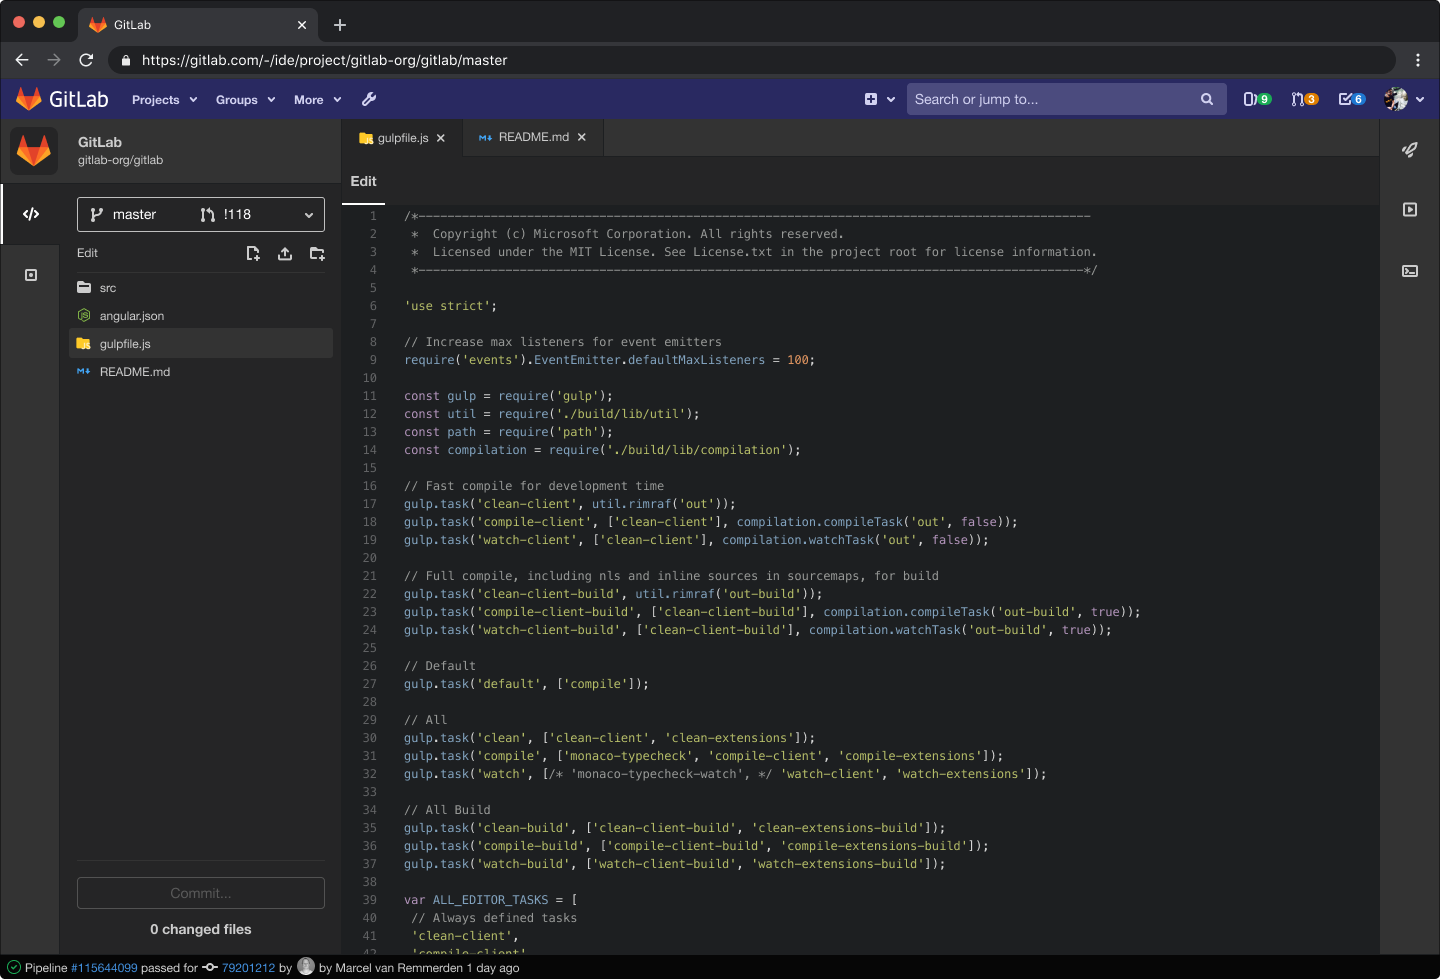
\includegraphics[width=.9\linewidth]{gorseller/gitlab-web-ide-karanlik-tema.png}
\caption{Tarayıcı üzerinden kod yazmaya olanak sağlayan GitLab Web IDE'de artık karanlık tema mevcut.}
\end{figure}
\newpage
GitLab 13.0 ile gelen diğer özellikler için konu başlığına eklediğim
bağlantıya tıklayabilirsiniz.
\section{Docker ve Snyk firmalarından konteyner güvenliği alanında \href{https://www.docker.com/press-release/Docker-Snyk-Announce-Partnership-Container-Vulnerability-Scanning}{iş birliği duyurusu}}
\label{sec:orgf626897}
Linux içerisindeki \texttt{cgroups} ile birlikte gelen konteyner sistemini
popülerleştirmesiyle bilinen Docker firması ve yazılımın çeşitli alanlarıyla
ilgili güvenlik çözümleri sunan Snyk şirketi, geçtiğimiz hafta içerisinde iş
birliği yaptıklarını duyurdular.

Bu iş birliği kapsamında Docker Hub sistemine eklenecek yeni bir entegrasyon
sayesinde artık Docker Hub'a gönderdiğimiz konteyner imajlarına otomatik
olarak güvenlik taraması yaptırabilir ve raporlayabilir olacağız.

Container teknolojisinin artan popülaritesi ile birlikte güvenlik
ihtiyaçlarının da aynı oranda artacağı tahmin edilebilir bir durum. Snyk
firması da bu alana erkenden giren firmalardan birisi olmuş.

Bu iş birliğinin ilk meyvelerini 2020'nin üçüncü yarısında görmeye
başlayacağız. Container teknolojisi ile ilgili arkadaşlara "Container
Security" alanına bakmalarını tavsiye ederim.
\section{Electron \href{https://www.electronjs.org/blog/electron-9-0}{9.0.0 sürümü yayınlandı}}
\label{sec:org512e157}
JavaScript kullanarak platformlar arası masaüstü uygulama geliştirmeye yarayan
kütüphane Electron, geçtiğimiz hafta içerisinde 9.0.0 etiketli sürümünü
yayınladı. Bu sürümle birlikte gelen bazı yenilik ve değişiklikler ise şöyle:

\begin{itemize}
\item Chromium sürümü 83.0.4103.64 olarak yükseltildi.
\begin{itemize}
\item \href{https://developers.google.com/web/updates/2020/04/nic81}{Chrome 81 sürüm notları}
\item Chrome 82 sürümü \href{https://chromereleases.googleblog.com/2020/03/chrome-and-chrome-os-release-updates.html}{koronavirüs nedeniyle atlandı}.
\item \href{https://developers.google.com/web/updates/2020/05/nic83}{Chrome 83 sürüm notları}
\end{itemize}
\item Node.js sürümü 12.14.1 olarak yükseltildi. \href{https://nodejs.org/en/blog/release/v12.14.1/}{Sürüm Notları}
\item V8 sürümü 8.3 olarak yükseltildi.
\begin{itemize}
\item \href{https://v8.dev/blog/v8-release-81}{V8 8.1 sürüm notları}
\item \href{https://v8.dev/blog/v8-release-83}{V8 8.3 sürüm notları}
\end{itemize}
\item İmla kontrolü özelliğinde iyileştirmeler: \href{https://github.com/electron/electron/pull/22128}{\#22128} ve \href{https://github.com/electron/electron/pull/22368}{\#22368}
\item Linux üzerinde Window Events Handler verimliliği iyileştirildi. (\href{https://github.com/electron/electron/pull/23260}{\#23260})
\item PDF görüntüleyici desteği geri geldi. (\href{https://github.com/electron/electron/pull/22131}{\#22131})
\item \texttt{enableRemoteModle: true} olmadan \texttt{remote} kullanılırsa artık deprecate
uyarısı veriyor. (\href{https://github.com/electron/electron/pull/21546}{\#21546})
\item \texttt{app.enableRendererProcessReuse} özelliği artık artık varsayılan olarak
\texttt{true}. (\href{https://github.com/electron/electron/pull/22336}{\#22336})
\item JavaScript olmayan objeleri IPC üzerinden gönderirken artık exception
fırlatıyor. (\href{https://github.com/electron/electron/pull/21560}{\#21560})
\end{itemize}

Bu sürümle gelen diğer yenilik ve değişiklikler için konu başlığına eklediğim
bağlantıya tıklayabilirsiniz.
\section{Windows Terminal \href{https://devblogs.microsoft.com/commandline/windows-terminal-1-0/}{1.0 sürümü yayınlandı} ve Windows Package Maganer Preview \href{https://devblogs.microsoft.com/commandline/windows-package-manager-preview/}{tanıtıldı}}
\label{sec:orgee60836}
Microsoft'un GNU/Linux ve MacOS taraflarına kaybettiği geliştirici kitlesini
geri kazanmak için yaptığı hamleler sürüyor. Uzun süredir geliştirilmekte
olan, benim de sık sık gündemde yer verdiğim Windows'un yeni Terminal'i
geçtiğimiz hafta düzenlenen BUILD 2020 etkinliğinde 1.0 olarak stabil
versiyonuna kavulmuş oldu.

\begin{figure}[htbp]
\centering
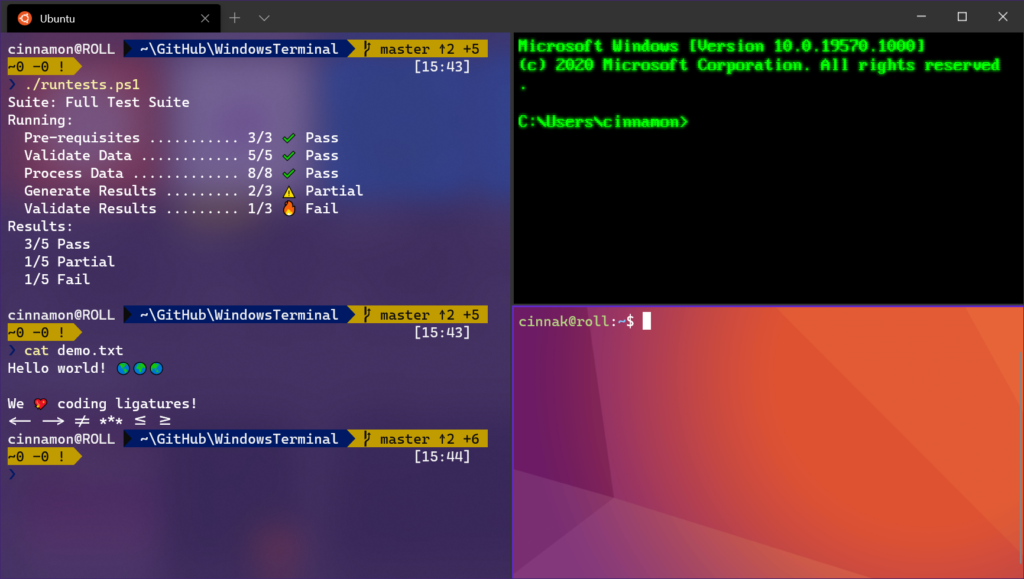
\includegraphics[width=.9\linewidth]{gorseller/windows-terminal-1-0.png}
\caption{Artık Windows üzerinde de gelişmiş bir terminal emülatörümüz mevcut.}
\end{figure}
\newpage

Önceki yazılım gündemi yazılarında zaten birçok Windows Terminal sürümününde
gelen yenilikleri konuşmuştuk. Bugün biraz daha önemli olduğunu düşündüğüm
\href{https://github.com/microsoft/winget-cli}{Windows Package Manager} üzerine konuşmak istiyorum.

\texttt{sudo apt install firefox}

Aramızdaki çoğu kişi yukarıda yazdığım komut satırı kodunun ne iş yaptığını
biliyor. Gerçi bilmeseniz bile ingilizce olarak okuduğunuzda zaten
anlaşılıyor. Firefox yazılımını sisteme kuruyor. İşte bu yapının benzeri artık
windows tarafında şu şekilde mevcut:

\begin{figure}[htbp]
\centering
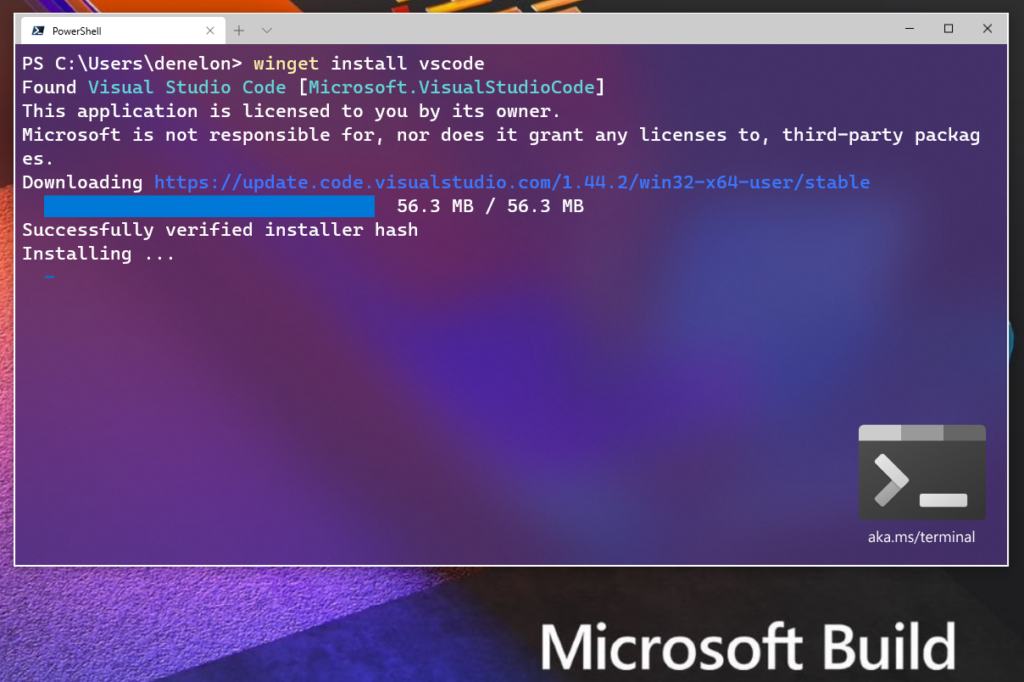
\includegraphics[width=.9\linewidth]{gorseller/winget-install.png}
\caption[\texttt{winget install firefox}]{\texttt{winget install firefox}}
\end{figure}
\newpage

Henüz ön izleme sürümü yayınlanmış bu paket yöneticisi Windows için oyun
değiştirici olma rolünü üstlenebilir. Şimdilik sadece \href{https://github.com/microsoft/winget-pkgs}{şu depodaki manifest
dosyaları} üzerinden exe dosyalarını indirip, çalıştırma görevi görüyor olsa da
hash doğrulama gibi önemli özellikleri de mevcut. Bence paket yöneticilerinin
en önemli özelliği \texttt{upgrade} komutu ile sistemde yüklü tüm uygulamaları tek
seferde güncelleyebilmek fakat bu henüz \texttt{winget}'e gelmiş değil. Bu özelliğin
kesinlikle getireceklerdir. Geliştirme ortamlarını Windows üzerinde kurmuş
birçok kişiye hatta son kullanıcıların bile çok işine yarayacağını
düşünüyorum.
\section{Yaklaşan Online Etkinlikler \#EvdeKal}
\label{sec:orge5fe42d}
\begin{longtable}{|p{9.5cm}|l|}
\hline
Etkinlik İsmi & Tarihi\\
\hline
\endfirsthead
\multicolumn{2}{l}{Önceki sayfadan devam ediyor} \\
\hline

Etkinlik İsmi & Tarihi \\

\hline
\endhead
\hline\multicolumn{2}{r}{Devamı sonraki sayfada} \\
\endfoot
\endlastfoot
\hline
\href{https://kommunity.com/pgtr/events/postgresql-sohbetleri-16-turkiyede-postgresql-ne-durumda-turker-gulum-587e9d43}{PostgreSQL Sohbetleri 16: Türkiye'de PostgreSQL ne durumda? (Türker Gülüm)} & 26 Mayıs 13:30\\
\href{https://kommunity.com/devops-turkiye/events/kubernetes-118de-gelen-yenilikler-3defef02}{Kubernetes 1.18'de gelen yenilikler} & 27 Mayıs 20:00\\
\href{https://kommunity.com/cloud-and-serverless-turkey/events/cloudflare-workers-just-write-code-54aace34}{Cloudflare Workers: Just Write Code} & 28 Mayıs 12:00\\
\href{https://kommunity.com/teknoloji-gelistirenler-icin-devlet-tesvikleri/events/mobil-uygulama-oyun-gelistirenler-icin-devlet-tesvikleri-111055dc}{Mobil Uygulama-Oyun Geliştirenler İçin Devlet Teşvikleri} & 28 Mayıs 14:00\\
\href{https://kommunity.com/bilisim-vadisi/events/google-cloud-gaming-ile-ilgili-cozumler-75d9af64}{Google Cloud Gaming ile İlgili Çözümler} & 29 Mayıs 13:00\\
\href{https://kommunity.com/tensorflow-turkey/events/contextual-chatbots-with-rasa-and-tensorflow-36eee01c}{Contextual chatbots with Rasa and TensorFlow} & 30 Mayıs 21:00\\
\href{https://kommunity.com/cloud-and-serverless-turkey/events/kubernetes-hands-on-4-kubernetes-ingress-and-network-policies-4f1cd707}{Kubernetes Hands-On no.4: Kubernetes Ingress and Network Policies} & 31 Mayıs 13:30\\
\hline
\end{longtable}
\section{Diğer Haberler}
\label{sec:orgcc072d3}
\begin{itemize}
\item GitHub, Go'nun MySQL sürücüsünde \href{https://github.blog/2020-05-20-three-bugs-in-the-go-mysql-driver/}{3 hatayı düzeltmiş.}.
\item Microsoft: "Açık Kaynak konusunda \href{https://www.zdnet.com/article/microsoft-we-were-wrong-about-open-source-but-luckily-you-can-change/}{yanıldık}." \href{https://www.theregister.co.uk/2020/05/15/microsoft\_brad\_smith\_open\_source/}{Alternatif}
\item Microsoft, Linux'e Direct3D 12 desteği \href{https://devblogs.microsoft.com/directx/directx-heart-linux/}{getireceğini açıkladı}. \href{https://www.phoronix.com/scan.php?page=news\_item\&px=Microsoft-DX12-WSL2}{Alternatif}
\item Defold oyun motoru \href{https://defold.com/opensource/}{açık kaynak hale geldi}. \href{https://github.com/defold/defold}{GitHub Deposu}
\item Microsoft klasik masaüstü uygulamalar ile UWP uygulamalarını \href{https://www.theverge.com/2020/5/19/21258697/microsoft-windows-project-reunion-win32-uwp-apps-apis-build}{birleştirmek
istiyor}: \href{https://github.com/microsoft/ProjectReunion}{Project Reunion}.
\item Visual Studio 2019 \href{https://docs.microsoft.com/en-us/visualstudio/releases/2019/release-notes-preview}{Preview 1 sürümü yayınlandı}.
\item Python programlama dilinin \href{https://pythoninsider.blogspot.com/2020/05/python-390b1-is-now-available-for.html}{3.9.0 Beta 1 sürümü yayınlandı}.
\item Node.js \href{https://nodejs.org/en/blog/release/v14.3.0/}{v14.3.0 sürümü yayınlandı}.
\item Deno \href{https://github.com/denoland/deno/releases/tag/v1.0.2}{v1.0.2 sürümü yayınlandı}.
\item F\# programlama dilinin \href{https://devblogs.microsoft.com/dotnet/f-5-update-for-net-5-preview-4/}{5.0 sürümü yayınlandı}.
\item Microsoft, \href{https://codeforces.com/blog/entry/77614}{Q\# Programlama Yarışması'nı duyurdu}.
\item Microsoft, GW-BASIC programlama dilinin \href{https://devblogs.microsoft.com/commandline/microsoft-open-sources-gw-basic/}{kodlarını açık kaynak yaptı}. \href{https://github.com/microsoft/GW-BASIC}{GitHub
Deposu}
\item Blazor WebAssembly kütüphanesinin \href{https://devblogs.microsoft.com/aspnet/blazor-webassembly-3-2-0-now-available/}{3.2.0 sürümü yayınlandı}.
\item Curl kullanıcı \href{https://daniel.haxx.se/blog/2020/05/18/help-curl-the-user-survey-2020/}{anketi başladı}. \href{https://forms.gle/4L4A2de4WgmJbJkg9}{Anket}
\item Grafana \href{https://grafana.com/blog/2020/05/18/grafana-v7.0-released-new-plugin-architecture-visualizations-transformations-native-trace-support-and-more/?isource=hp}{v7.0 sürümü yayınlandı}.
\item PostgreSQL \href{https://www.postgresql.org/about/news/2040/}{13 Beta 1 sürümü yayınlandı}.
\item SQLite \href{https://sqlite.org/releaselog/3\_32\_0.html}{3.32.0 sürümü yayınlandı}.
\item Beekeeper Studio \href{https://www.beekeeperstudio.io/blog/release-1.4}{1.4 sürümü yayınlandı}.
\item Orx oyun motorunun \href{https://www.gamedev.net/news/orx-portable-game-engine-version-111-has-been-released-r1349/}{1.11 sürümü yayınlandı}.
\item EA, Command\&Conquer ve Red Alert'in \href{https://kotaku.com/ea-is-releasing-command-conquer-and-red-alerts-source-1843574798}{kaynak kodlarını yayınlayacak}.
\item Swift programlama dili için fonksiyonel mimari çözümü sunan \href{https://www.47deg.com/blog/bow-arch-0-1-0-release/}{açık kaynaklı
kütüphane tanıtıldı}: \href{https://arch.bow-swift.io/}{Bow Arch}. \href{https://github.com/bow-swift/bow-arch}{GitHub Deposu}
\item tree-hugger açık kaynaklı \href{https://medium.com/codist-ai/introducing-tree-hugger-source-code-mining-for-human-b5fcd31bef55}{projesi tanıtıldı}. \href{https://github.com/autosoft-dev/tree-hugger}{GitHub Deposu}
\item GrallVM \href{https://www.graalvm.org/docs/release-notes/20\_1/}{20.1.0 sürümü yayınlandı}.
\end{itemize}
\section{Lisans}
\label{sec:org144f608}
\begin{center}
\begin{center}

\includegraphics[height=1.5cm]{../../../img/CC_BY-NC-SA_4.0.png}
\end{center}

\href{yazilim-gundemi-2020-20.pdf}{Yazılım Gündemi - 2020/20} yazısı \href{https://erenhatirnaz.github.io}{Eren Hatırnaz} tarafından \href{http://creativecommons.org/licenses/by-nc-sa/4.0/}{Creative Commons
Atıf-GayriTicari-AynıLisanslaPaylaş 4.0 Uluslararası Lisansı} (CC BY-NC-SA 4.0)
ile lisanslanmıştır.
\end{center}
\end{document}
